\documentclass[tikz]{standalone}
\tikzset{
  >=latex
}

\begin{document}
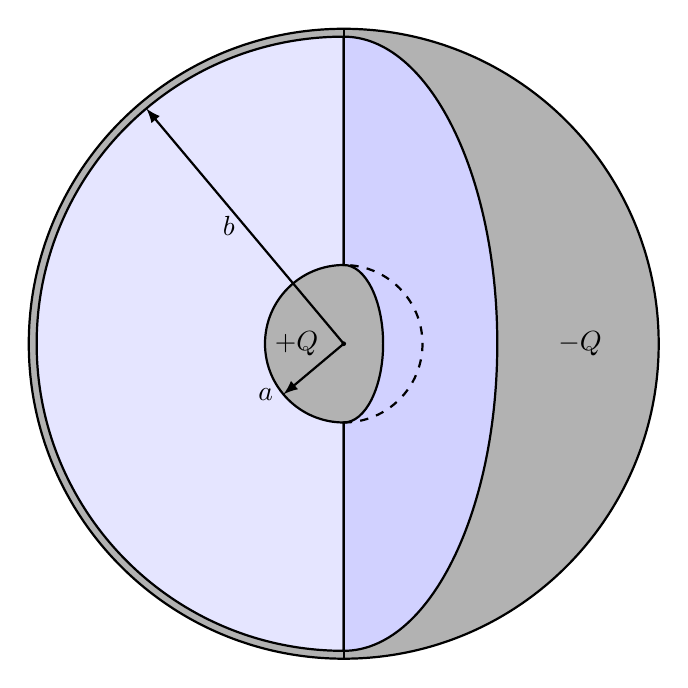
\begin{tikzpicture}
  \draw[thick,fill=gray!60](0,0) circle(4);
  \draw[thick,fill=blue!10](0,3.9) arc(90:270:3.9)--(0,-1)
  arc(270:90:1)--(0,3.9);
  \draw[thick,fill=blue!18] (0,3.9)arc(90:-90:1.95 and 3.9)--(0,-1)
  arc(-90:90:.5 and 1)--(0,3.9);
  \draw[thick,dashed](0,-1) arc(-90:90:1);
  \draw[thick,->,rotate=-50](0,0)--(-3.9,0) node[midway,left]{$b$};
  \draw[thick,->,rotate=40](0,0)--(-1,0) node[left]{$a$};
  \fill(0,0) circle(.03);
  \draw[thick] (0,3.9)--(0,4);
  \draw[thick] (0,-3.9)--(0,-4);
  \node at (3,0) {$-Q$};
  \node at (-.6,0) {$+Q$};
\end{tikzpicture}
\end{document}
